A key goal of our parallel design is to keep the threads as busy as possible and
to reduce inter-thread communication. Initially, the VM partitions the
application graph of $N$ nodes into $T$ subgraphs (the number of threads) and
then each thread works on their own subgraph. During execution, threads can
steal nodes of other threads to keep themselves busy. The load balancing aspect
of the system is performed by our work scheduler that is based on a simple work
stealing algorithm.

While our VM uses shared memory for thread communication, each
thread has a logical space that contains its subgraph, i.e., the nodes owned by
the thread, and a \emph{Work Queue}, which contains \textbf{active} nodes, i.e.,
nodes that have new facts to process.  The work queue is implemented as a linked
list. Initially, the work queue is filled with the nodes in the thread's
subgraph in order to derive the initial facts. A thread may go through different
states during its lifetime. The state is kept track in the \emph{State} flag
which may have one of the following values:

\begin{itemize}

   \item \textbf{active}: The thread has a non-empty \emph{Work Queue} or is
      currently executing rules for a node (which is not in the \emph{Work
      Queue}).

   \item \textbf{stealing}: The thread has no active nodes in the \emph{Work
      Queue} and is attempting to steal nodes from other
      threads.

   \item \textbf{idle}: The thread is trying to synchronize with other threads
      to terminate the program.
   
   \item \textbf{terminated}: The thread (and all the other threads) have
      terminated and the program is finished.

\end{itemize}

Figure~\ref{fig:implementation:thread_states} presents the valid transitions for
the thread state flag. The dashed line from \textbf{idle} to \textbf{stealing}
indicates that the transition is made in a non-deterministic fashion.

\begin{figure}[ht]
   \centering
   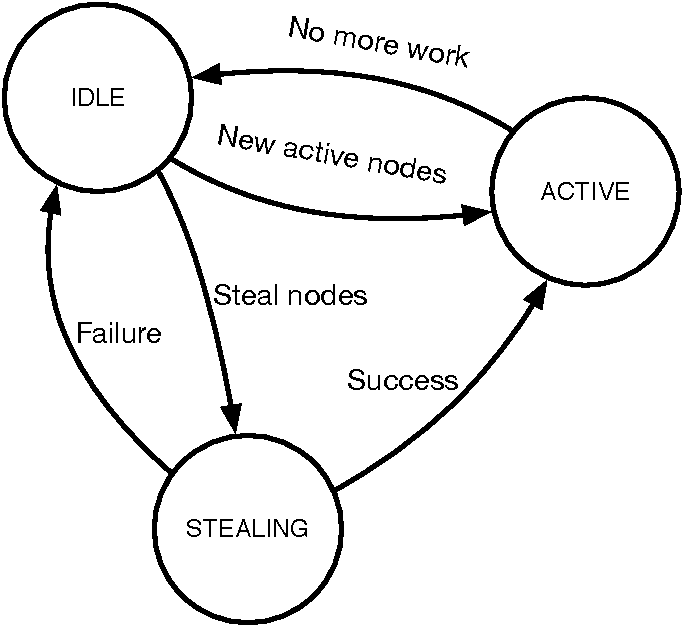
\includegraphics[width=0.65\textwidth]{figures/implementation/thread_states.pdf}
   \caption{The thread state machine as represented by the \emph{State} flag. During
      the lifetime of a program, each thread goes through different states as
      specified by the state machine.}
   \label{fig:implementation:thread_states}
\end{figure}

The pseudo-code for the main thread loop is shown in
Fig.~\ref{alg:thread_work_loop}. In each round, a thread inspects its \emph{Work
Queue} and while there are active nodes, procedure \code{process\_node()}
(complete pseudo-code in Fig.~\ref{alg:multicore:process_node}) will perform
local computation on active nodes. When a thread's \emph{Work Queue} is empty,
it attempts to steal half of the nodes from another thread. Starting from a
random thread, it cycles through all the threads to find one active thread from
whom it will try to steal half of its nodes. If the thread fails to steal work,
it will go \textbf{idle} and periodically attempt to steal work from another
active thread. Eventually, all threads will fail to steal work since there is no
more work to do and they will go idle.  There is a global atomic counter that is
used to detect termination. Once a thread goes idle, it decrements the global
counter and changes its flag to idle.  Since every thread will be busy-waiting
and checking the global counter, they will detect a zero value and stop
executing, transitioning to the \textbf{terminated} state.

\begin{figure}
\begin{algorithm}[H]
   \KwData{Thread TH}
   \While{true}{
      $TH.work\_queue.lock()$\;
      $node \longleftarrow TH.work\_queue.pop\_node()$ \;
      $TH.work\_queue.unlock()$\;
      \uIf{$node$}{
         $process\_node(node)$\;
      }
      \Else{
         \tcc{Attempt to steal some nodes.}
         \If{$\bang TH.steal\_nodes()$}{
            $TH.become\_idle()$\;
            \While{$len(TH.work\_queue) == 0$}{
               \tcc{Try to terminate}
               \If{$TH.synchronize\_termination()$}{
                  \textbf{terminate}\;
               }
               \If{$TH.steal\_nodes()$}{
                  \tcc{Thread is still in the stealing state}
                  break\;
               }
            }
            \tcc{There's new nodes in the queue.}
            $TH.become\_active()$\;
         }
      }
 }
\end{algorithm}
\caption{Thread work loop: threads process active nodes from the work queue
   until no more active nodes are available. Node stealing using a \emph{steal
      half} strategy is employed when the thread has no more active nodes.}
 \label{alg:thread_work_loop}
\end{figure}

Figure~\ref{fig:implementation:vm_overview} ties everything together and
presents the layout of our virtual machine for a program with six nodes and two
running threads. In the figure, we represent the thread's \emph{Work Queue} and
the thread logical space where the thread's subgraph is located. We also show
the internals of node \code{@1} and the thread operations that force threads to
interact with the node data structures.

\begin{figure*}[t]
\centering
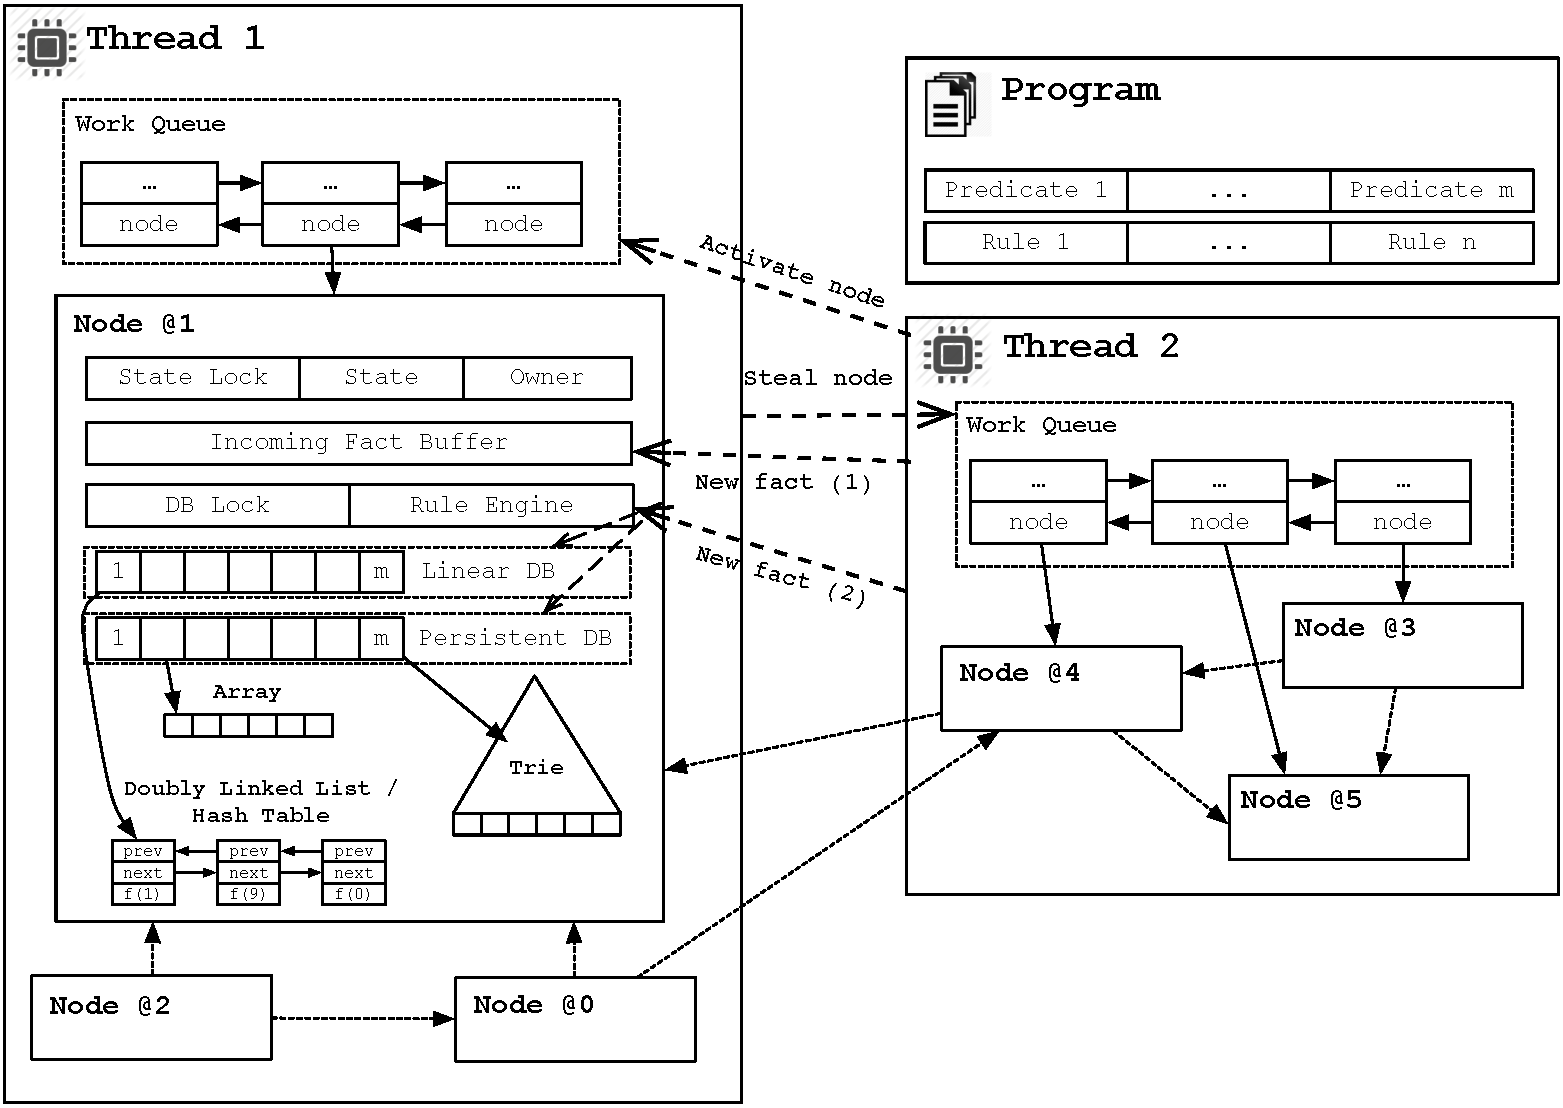
\includegraphics[width=\textwidth]{figures/implementation/vm_overview.pdf}
\caption{Layout of the virtual machine. Each thread has a work queue that
   contains active nodes (nodes with facts to process) that are processed one
   by one by the thread. Communication between threads happens when nodes
   send facts to nodes located in other threads.}
\label{fig:implementation:vm_overview}
\end{figure*}

In order to understand how threads interact between each other, we now review
the node data structure that was presented in Section~\ref{sec:data_structures}.
The node lock \emph{DB Lock} protects the data structures of the database,
including the array, trie, linked list and hash table data structures and the
\emph{Rule Engine}. The \emph{State Lock} structure protects everything else,
especially the \emph{State} flag and the temporary set of facts represented by
the \emph{Fact Buffer}. The \emph{Incoming Fact Buffer} is used to hold logical facts
that can not be added immediately to the database data structures. The
\emph{Owner} field points to the thread responsible for processing the node and
the \emph{Rule Engine} schedules local computation.

Whenever a new fact is derived through rule derivation, we need to update the
data structures for the corresponding node. If the node is currently being
executed by the thread (local send), then the fact is added to the node data
structures since the \emph{DB Lock} is being held while the node is being
processed. If that is not the case, then we have to synchronize since multiple
threads might be updating the same node's data structures. For example, in
Fig.~\ref{fig:implementation:vm_overview}, when thread 2 derives a fact to node
\code{@1} (owned by thread 1), it first locks node \code{@1} using the
\emph{State Lock} and then it attempts to lock \emph{DB Lock}, which gives thread
2 full access to the node. In this case, thread 2 adds the new fact to the
database (\emph{New fact (2)} in Fig.~\ref{fig:implementation:vm_overview}) and
to the \emph{Rule Engine}. However, if the \emph{DB Lock} could not be acquired
because the node \code{@1} is currently being processed, then the new fact is
added to \emph{Incoming Fact Buffer} (\emph{New fact (1)} in
Fig.~\ref{fig:implementation:vm_overview}). The facts stored in \emph{Fact
Buffer} will then be processed whenever the corresponding node is processed
again.

When a thread interacts with another thread to send a fact, it also needs to
make sure that the target node is made \textbf{active} (see
Fig.~\ref{fig:local:node_states}) and that it is also placed in the target
thread's \emph{Work Queue} (\emph{Activate node} in
Fig.~\ref{fig:implementation:vm_overview}). To handle concurrency issues, we
have a per \emph{Work Queue} lock called the \emph{Queue Lock} that is held when
the \emph{Work Queue} is being operated on.  As an example, consider again the
situation in which thread 2 sends a new fact to node \code{@1}. If node
\code{@1} is not active, then thread 2 also needs to activate node \code{@1} by
pushing it to the \emph{Work Queue} of thread 1.  After this synchronization
point, the target thread is ensured to be active and with a new node to process.

\begin{figure}
\begin{algorithm}[H]
   \KwData{Node N}
   $N.state\_lock.lock()$\;
   $N.db\_lock.lock()$\;
   \tcc{Add facts from the Incoming Fact Buffer into the database}
   $N.DB.merge(N.incoming\_fact\_buffer)$\;
   $N.state\_lock.unlock()$\;

   $N.rule\_engine.run\_rules()$\;
   $N.db\_lock.unlock()$\;

   \tcc{Check if node N is done for now}

   $N.state\_lock.lock()$\;
   \If{$N.rule\_engine.has\_candidate\_rules()$ or \\
      \hspace{2cm} $N.incoming\_fact\_buffer.has\_facts()$}{
      $N.state\_lock.unlock()$\;
      goto beginning\;
   }
   $N.state \longleftarrow inactive$\;
   $N.state\_lock.unlock()$\;
\end{algorithm}
\caption{Pseudo-code for the \code{process\_node} procedure.}
 \label{alg:multicore:process_node}
\end{figure}
